%%%%                %%%%
%%%% IMPLEMENTACIÓN %%%%
%%%%                %%%%

\chapter{Implementación}
\label{chap:implemetación}

La implementación está diseñada para recibir peticiones de conversión y generar la salida correspondiente en formato estructurado. El número de ficheros que se pueden tratar en cada ejecución solo está limitado por las capacidades del sistema operativo donde se ejecute. Cada invocación crea una tarea en el sistema, que se gestiona de forma individual. Una vez que se reciben los ficheros para su tratamiento, se produce una ruta específica para ese trabajo y comienza el proceso. En cada etapa se crean nuevos ficheros intermedios que, según se verá más adelante, se mueven a destinos designados para cada paso. El motor encargado de conducir el flujo de información está implementado en lenguaje Bash. El \emph{engine} utiliza varias herramientas complementarias, disponibles en cualquier distribución Linux. Se complementan con el generador de código intermedio y los parsers para cada modelo de documento.

Existen, por tanto, tres partes que se detallarán en las siguientes páginas:

\begin{itemize}
    \item Un motor o \emph{engine} creado con \emph{scripts} en lenguaje Bash. Su cometido es recepcionar los ficheros y transformarlos paso a paso hasta la obtención de la salida final.
    \item Una aplicación Python encargada de generar el lenguaje intermedio que va a ser procesado.
    \item Una familia de escáners y parsers desarrollados empleando Flex \cite{estes_flex_2021} y GNU Bison \cite{free_software_foundation_inc_bison_nodate}. Toman como entrada el lenguaje intermedio y lo traducen a un formato estructurado.
\end{itemize}

Se describen a continuación cada una de ellas.

\section{El engine}
La herramienta se planteó como un software que pudiera ser capaz de recibir uno o varios ficheros en cada invocación. Una vez recibido, cada input debía ser clasificado e identificado para su correcto tratamiento. Dado que la entrada y la salida serían ficheros, resultaba natural utilizar un lenguaje de programación con facilidades para la manipulación de ficheros. Por ser el entorno de operación y desarrollo un sistema GNU/Linux, se optó por emplear el intérprete de \emph{shell} Bash.

Por tratarse de un conjunto de \emph{scripts}, este \emph{pipeline} es flexible tanto para añadir nuevos pasos como para quitarlos. La razón para hacerlo de este modo radica en posibilitar la incorporación de nuevas técnicas de procesado de cualquiera área relevante, como el tratamiento de imagen o la extracción de texto. Cada \emph{script} es independiente y puede ser ser activado o desactivado fácilmente.

%% Convenio de nombrado para evitar perder información o mezclar páginas

%% Elaboración de las plantillas: Las plantillas son ficheros en formato JSON. Contienen las coordenadas de la geometría para las regiones de interés.

%% Generación del lenguaje intermedio: el sistema de generación de lenguaje intermedio debía ser necesariamente flexible. Para poder aplicar técnicas distintas. Se optó por utilizar Python, que tiene mucho soporte y una gran colección de librerías disponibles.

%% Detección de subregiones: Se diseñó un algoritmo sencillo pero eficaz para decidir si una región era subregión de otra dada.

%% Aproximación para la identificación de las lineas individuales: Esta aproximación se basó en intentar caracterizar las lineas mediante propiedades sencillas. La aproximación no dio resultado.

%% Mejora de tiempos: Inicialmente se utilizada el tipo de dato Set y sus operaciones para comprobar la inclusión de unas regiones en otras. Esta aproximación, aunque funcional, no resultaba rápida para su ejecución durante el desarrollo. Se realizó una mejora que comprueba las propiedades geométricas en lugar de basarse en lógica de conjuntos.

%% Obtención de información estructurada
%%%% Flex
%%%% Bison

%% Despliegue de la aplicación

%% Cambios para integrarse con la GUI
%%%% Exponiendo las coordenadas 
%%%% Uso de Docker

\section{Estructura física}

Para entender más fácilmente las características de la implementación se describen primero la estructura de directorios que conforman el proyecto. La aplicación se compila y distribuye por medio de un \verb|Makefile|. También se implementó un fichero \verb|Dockerfile| configurado para generar la correspondiente imagen Docker del programa. 
La estructura y funcionalidad de los directorios del proyecto es importante para detallar como se trata la entrada. Esta estructura general se puede consultar gráficamente en XXX. Los principales directorios utilizados son:

\begin{itemize}
    \item \verb|conf|, empleado para las configuraciones del \emph{engine}, también la configuración de Tesseract y los datos de entrenamiento.
    \item \verb|data| contiene información de los modelos soportados. Principalmente los identificadores utilizados para reconocer los documentos y las plantillas que relacionan las regiones seleccionadas.
    \item \verb|doc| está dedicado a la documentación del proyecto y a esta memoria, escrita en formato \LaTeX. También contiene todos los ejemplos de ficheros PDF utilizados.
    \item \verb|engine| tiene como finalidad alojar todos los \emph{scripts} del \emph{engine}.
    \item \verb|input| no está en el repositorio, sino que se crea bajo demanda, es la ruta base para la entrada de datos utiliza por la aplicación. El nombre se escoge en la configuración del \emph{engine}.
    \item \verb|script| mantiene varios \emph{scripts} auxiliares utilizados principalmente para facilitar las ejecuciones durante el desarrollo.
    \item \verb|tool-gen-language| es la carpeta dedicada a los fuentes de la herramienta de generación de lenguaje intermedio.
    \item Por último, \verb|tool-parser| contiene la aplicación Flex/Bison y los \verb|plugins| que convierten el lenguaje intermedio a la salida JSON.
\end{itemize}

\section{Tratamiento inicial de la entrada}

La herramienta es un software \verb|backend|, no está pensada para que un usuario realice las ejecuciones de la aplicación manualmente. Por ello, y aunque no se desarrolló un API para acompañar la solución, si que se definieron varias características con la finalidad de facilitar la depuración durante el desarrollo y servir de primera aproximación para una futura integración en un sistema con un diseño por capas.

Cada ejecución se lleva a cabo en un directorio propio donde se almacena la entrada, se realiza el tratamiento y se ubica la salida. Además se facilita al programa llamante un identificador que debe utilizar para la recuperación de los resultados. La ruta al directorio que contiene todas las carpetas de todas las ejecuciones el es directorio \verb|input|, mencionado anteriormente.

Para evitar colisiones en las rutas de trabajo entre distintas ejecuciones se obtiene una marca de tiempo del instante de recepción de la petición. Para obtener este \emph{timestamp} se utiliza el comando \verb|date| de la forma siguiente:

\begin{verbatim}
diego@CompaqCQ57:galiasdoc$ date -u +"%s%6N"
1616623143141490
diego@CompaqCQ57:galiasdoc$
\end{verbatim}

A continuación se presenta la secuencia de pasos que conforman en comienzo de una tarea en el sistema. La primera acción ocurre cuando el invocador del sistema ejecuta el \emph{script} \verb|get-job-id.sh|. Este crea el nuevo directorio para el trabajo y todos los directorios internos. Se devuelve el identificador de trabajo al llamador.

En este momento el llamador debe copiar el fichero de entrada en la ruta \verb|job_id/frontend|. Por último se inicia la ejecución cuando se llama al \emph{script} \verb|run.sh|. La entrada que habrá de tratar se indica con el \verb|job_id| pasado como parámetro. Los pasos se pueden seguir visualmente en la figura \ref{fig:inicio-aplicacion}.

A partir de este momento el sistema comienza a trabajar. Cada acción llevada a cabo se indica con un mensaje por la salida estándar de la consola. Cuando finaliza se notifica con otra marca de tiempo del momento final en la ruta \verb|input/job_id/done-<timestamp>|.

\begin{figure}[hp!]
  \centering
  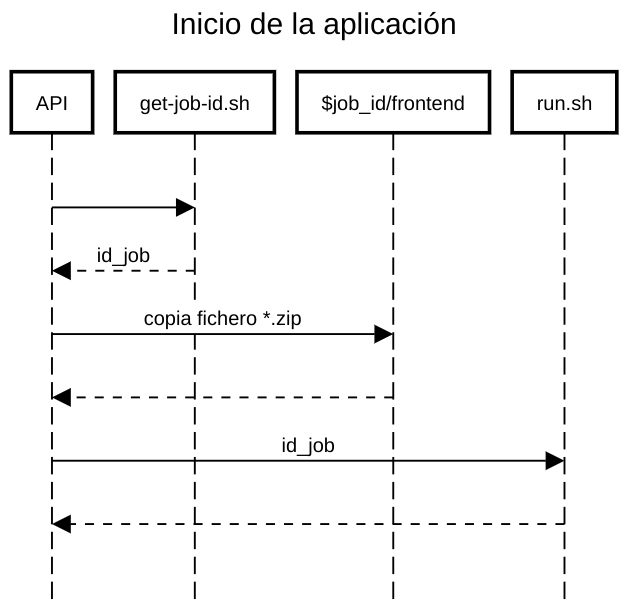
\includegraphics[width=11cm]{imaxes/inicio-aplicacion.png}
  \caption{Secuencia de inicio de la aplicación}
  \label{fig:inicio-aplicacion}
\end{figure}

%% Cambiar diagrama con flecha saliente para indicar que se ejecutan los pasos del engine
%% Cambiar "copia fichero *.zip" por "datos entrada"
%% La linea de finalización debe devolver el evento de finalización

\section{Flujo del engine}

Cuando se invoca el \emph{script} \verb|run.sh| se realizan en secuencia todos los pasos que acaban generado la salida en formato estructurado.

\begin{enumerate}
    \item Descompresión de la entrada.
    \item Renombrado seguro de los ficheros.
    \item Extracción de texto con \emph{pdftotext}.
    \item Clasificación de los casos basados en texto y aquellos basados en imagen.
    \item Generación de imágenes para los documentos basados en texto.
    \item Aplicación del OCR para los casos basados en imagen.
    \item Identificación de cada documento.
    \item Generación del lenguaje intermedio.
    \item Invocación del parser necesario.
    \item Publicación de los resultados en el directorio de salida.
\end{enumerate}

\section{Generación del lenguaje intermedio}
\section{Salida en lenguaje estructurado}